\documentclass[diploma]{nanolab2015}

\begin{document}
\begin{titlepage}
\begin{center}
    \large
    ФЕДЕРАЛЬНОЕ ГОСУДАРСТВЕННОЕ БЮДЖЕТНОЕ ОБРАЗОВАТЕЛЬНОЕ УЧРЕЖДЕНИЕ ВЫСШЕГО ОБРАЗОВАНИЯ «МОСКОВСКИЙ ГОСУДАРСТВЕННЫЙ УНИВЕРСИТЕТ ИМЕНИ М.В.ЛОМОНОСОВА»
     
    \textbf{Физический факультет}\\
    \vspace{4cm}
    \textsc{\Large Отчет по практическому заданию №4 (2.7(3))}\\[5mm]
    {\LARGE Численные методы в физике.}
\end{center}
\vspace{7cm}
\null
\begin{flushright}
\normalsize студента 427 группы
\\Шилина Максима Александровича
\end{flushright}
\vfill
\begin{center}
\textbf{Москва - 2022}
\end{center}
\end{titlepage}

\tableofcontents{}  % оглавление
\newpage

\section{Постановка задачи}
Численно решить, представленное ниже, уравнение теплопроводности на отрезке $x = [0,10]$ и интервале времени $t=[0,1]$ по явной схеме и по схеме Кранка-Николсона.
\begin{equation*}
\begin{cases}
   \frac{\partial T}{\partial t} = \frac{\partial^2 T}{\partial x^2}\\
   T(x=0, t)=T(x=10, t) = 0\\
   T(x, t=0) = \frac{41}{15} (x-5)^2 e^{-(x-5)^2}
 \end{cases}
\end{equation*}

Необходимо рассмотреть два варианта шагов интегрирования:

1) $dx = 0.1, dt = 0.01$

2) $dx = 0.1, dt = 0.005$

Необходимо построить графики T(x) для шести моментов времени, а также графики сеточной диффузии.

\section{Дисперсия точного уравнения}
Для нахождения дисперсионного соотношения необходимо подставить в исходное уравнение решение в виде плоской гармонической волны:

$$T(x,t) = T_0 e^{i(\omega t - \kappa x)}$$

После подстановки в уравнение получим чисто мнимое дисперсионное соотношение:

$$i \omega = -\kappa ^2$$

Это означает, что в задаче присутствует диффузия и полностью отсутствует дисперсия.

Чтобы получить действительное дисперсионное соотношение введём замену переменных: $i \omega = \delta$. Тогда вид решения и  дисперсионное соотношение примут следующий вид:

$$T(x,t) = T_0 e^{-\delta t - i \kappa x)}$$

$$\delta = - \kappa^2$$

\section{Исследование явной схемы}
Ниже представлена явная схема для решения уравнения теплопроводности:

$$\frac{T^{n+1}_{j}-T^{n}_{j}}{\Delta t}=\chi \frac{T^{n}_{j+1}-2T^{n}_{j}+T^{n}_{j-1}}{\Delta x^2}$$

Данная схема имеет первый порядок аппроксимации по t и второй порядок по координате x. Разностное уравнение можно переписать в более удобном виде, введя коэффициент $\alpha = \frac{\chi \Delta t}{\Delta x^2}$:

$$T^{n+1}_{j} = T^{n}_{j} + \alpha (T^{n}_{j+1} -2T^{n}_{j}+T^{n}_{j-1})$$

\begin{figure}[h!]
\centering
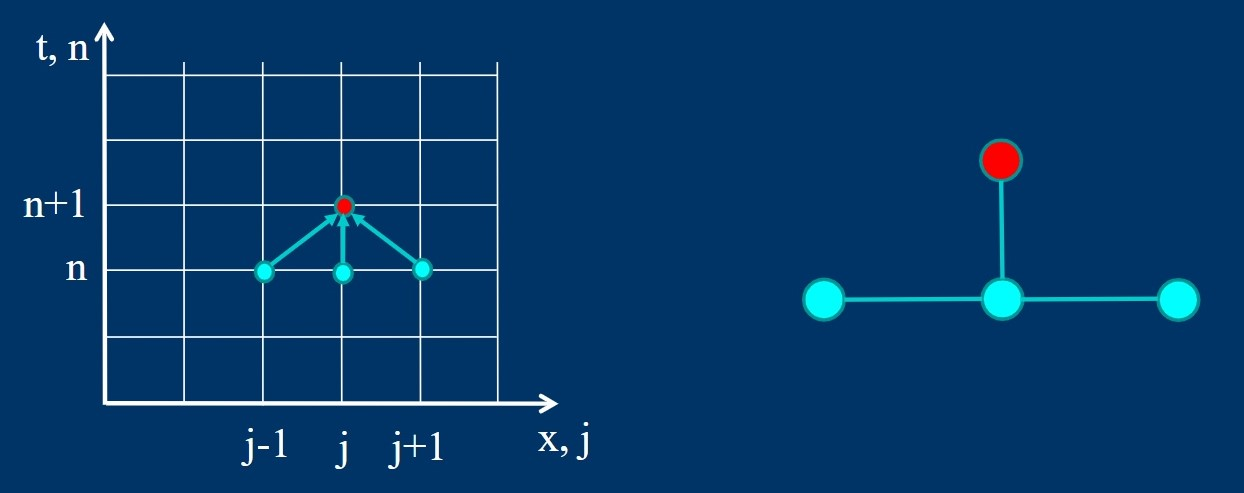
\includegraphics[scale=0.5]{scheme1.jpg}
\caption{\label{pic1}  Шаблон явной схемы. Красная точка - неизвестное значение функции в заданной точке. }
\end{figure}

\subsection{Условие устойчивости}
Для исследования устойчивости явной схемы рассмотрим пространственную Фурье-моду: $\hat{T}^n_\kappa e^{i \kappa x_j}$. Множитель перехода определяется следующим выражением: $\hat{T}^{n+1}_\kappa e^{i \kappa x_j}=\lambda \hat{T}^n_\kappa e^{i \kappa x_j}$. Подставим данные уравнения в разностную схему:

$$\lambda \hat{T}^n_\kappa e^{i \kappa x_j} = \hat{T}^n_\kappa e^{i \kappa x_j} + \alpha(\hat{T}^n_\kappa e^{i \kappa (x_j+\Delta x)} -2\hat{T}^n_\kappa e^{i \kappa x_j}+\hat{T}^n_\kappa e^{i \kappa (x_j-\Delta x)})$$

После преоброзований окончательно получим выражение для множителя перехода:

$$\lambda = 1 - 2\alpha(1-\cos(\kappa \Delta x))=1-4\alpha \sin^2\frac{\kappa \Delta x}{2}$$

Условием устойчивости является выполнение неравенства $|\lambda| \leq 1$. Для явной схемы это условие можно переписать в следующем виде:

$$4\alpha \sin^2\frac{\kappa \Delta x}{2} \leq 2$$, $$\alpha \leq \frac{1}{2}$$

Таким образом явная схема является условно устойчивой с условием на шаг: $\Delta t \leq \frac{\Delta x^2}{2 \chi}$.

Получив данное условие устойчивости можно сделать вывод, что в исследуемой задаче для шагов сетки  $dx = 0.1, dt = 0.01$ ожидается быстро нарастающая экспоненциальная неустойчивость решения, т.к.$\alpha = 1$, что довольно сильно больше 0,5. Шаги сетки $dx = 0.1, dt = 0.005$ лежат на границе устойчивости, а это значит, что можно ожидать устойчивого решения.

\subsection{Дисперсионное соотношение}
Можно довольно просто получить связь между множителем перехода и дисперсией:

$$T(x,t)=T_0 e^{-\delta t - i \kappa x}$$

$$\hat{T}^{n+1}_\kappa = \lambda \hat{T}^{n}_\kappa$$ 

Тогда получим, что

$$T_0 e^{-\delta (t_n+\Delta t) - i \kappa x_n}= \lambda T_0 e^{-\delta t_n - i \kappa x_n}$$

Откуда получаем искомое соотношение: $\delta \Delta t = - ln \lambda$. 

В общем случае $\delta$ - комплексное число, а значит, его можно представить в следующем виде: $\delta = \Gamma - i \Omega$.

$$\delta \Delta t = -ln|1-4\alpha \sin^2\frac{\kappa \Delta x}{2}|-i \pi=(\Gamma - i \Omega)\Delta t$$

$$\Gamma \Delta t = - ln|1-4\alpha \sin^2\frac{\kappa \Delta x}{2}|=- ln|1-4\alpha \sin^2\frac{\kappa \pi}{2 \kappa_N}|$$

Где $\kappa_N = \frac{\pi}{\Delta x}$ - волновой вектор Найквиста. Вводя безразмерный параметр $y$ можно записать соотношение в следующем виде:

$$\Gamma \Delta t = - ln|1-4\alpha \sin^2\frac{\pi y}{2}|$$

$\Gamma \Delta t$ - интересующая нас диффузия сеточного решения.

\section{Схема Кранка-Николсона}
Данная схема является симметричной схемой с весами второго порядка точности по времени и координатам. Рассмотрим её схему:

$$T^{n+1}_{j} = T^{n}_{j} + \frac{\alpha}{2} (T^{n}_{j+1} -2T^{n}_{j}+T^{n}_{j-1})+\frac{\alpha}{2} (T^{n+1}_{j+1} -2T^{n+1}_{j}+T^{n+1}_{j-1})$$

Видно, что данная схема является неявной.

\subsection{Устойчивость схемы}
Для исследования устойчивости явной схемы рассмотрим пространственную Фурье-моду: $\hat{T}^n_\kappa e^{i \kappa x_j}$. Множитель перехода определяется следующим выражением: $\hat{T}^{n+1}_\kappa e^{i \kappa x_j}=\lambda \hat{T}^n_\kappa e^{i \kappa x_j}$. Подставим данные уравнения в разностную схему:

$$\lambda \hat{T}^n_\kappa e^{i \kappa x_j} = \hat{T}^n_\kappa e^{i \kappa x_j}(1+\frac{\alpha}{2}(e^{i \kappa \Delta x}-2+e^{-i \kappa \Delta x})+\lambda \frac{\alpha}{2}(e^{i \kappa \Delta x}-2+e^{-i \kappa \Delta x}))$$

После преобразований получим следующее выражение для множителя перехода:

$$\lambda = \frac{1-2\alpha \sin^2 \frac{\kappa \Delta x}{2}}{1+2\alpha \sin^2 \frac{\kappa \Delta x}{2}}$$

Видно, что для любого $\alpha \geq 0$ $|\lambda| \leq 1$, это означает, что схема является абсолютно устойчивой.

\subsection{Дисперсионное соотношение}
Для нахождения дисперсии воспользуемся полученной ранее формулой: $\delta \Delta t = - ln \lambda$. 

$$\delta \Delta t = ln \left( \frac{1+2 \alpha \sin^2 \frac{\kappa \Delta x}{2}}{1-2 \alpha \sin^2 \frac{\kappa \Delta x}{2}}\right)$$

Выделяя действительную часть выражения, получим диффузию сеточного решения:

$$\Gamma \Delta t = ln \left(\frac{1+2 \alpha \sin^2 \frac{\kappa \Delta x}{2}}{|1-2 \alpha \sin^2 \frac{\kappa \Delta x}{2}|}\right)$$

Важной особенностью обеих схем является то, что при определённом значении параметра $\alpha$ появляется дисперсия решения, что не наблюдается в точном решении.

\subsection{Решение системы арифметических уравнений}
Преобразование схемы сводит исходную задачу к решению следующей системы уравнений:

$$a_j u_{j+1} +b_j u_j + c_j u_{j-1}=f_j$$

Где $a_j=c_j=1$, кроме двух значений $a_N=c_1=0$, $b_j=-2(1+1/ \alpha)$, а правая часть равна: $f_j = -T^{n}_{j+1} + 2(1-1/ \alpha)T^{n}_{j}-T^{n}_{j-1}$.

Ищем решение в виде: $u_{j+1} = x_{j}u_{j}+y_{j}$. Подставляя решения в исходное уравнение, получаем рекуррентные формулы для определения прогоночных коэффициентов:

$$x_{j-1} = -\frac{c_j}{b_j+a_j x_j}, \ j=2,...,N$$

$$y_{j-1}=\frac{f_j-a_j y_j}{a_j x_j + b_j}, \ j=2,...,N$$

Из рекуррентных формул находим (прямая прогонка) $x_j, y_j$.  Далее производим обратную прогонку: $u_{j+1} = x_{j}u_{j}+y_{j}$ и находим все $u_j$ решения линейной системы уравнений на данном временном слое.

Этот метод уникален тем, что арифметическая сложность данного алгоритма пропорциональна количеству неизвестных $O(N)$, в то время, как арифметическая сложность метода Гаусса пропорциональна квадрату количества неизвестных $O(N^2)$.

\section{Численное решение}
Языком для реализации численного метода выбран Python и библиотеки numpy и matplotlib. Для наглядности графики сделаны для 6 различных времён времени t и в 3D. Также была создана анимация решения.

На графиках, изображённых на рисунке \ref{pic2} видна теоретически  предсказанная экспоненциальная неустойчивость для первого выбора шагов, а так же сходимость для второго набора шагов. Также на рисунке \ref{pic4} видно, что решение ведёт себя устойчиво на отрезке времени 0-0.2 секунды.

Решение же по схеме Кранка-Николсона является абсолютно устойчивой схемой, что подтверждает графики на рисунке \ref{pic3}.

\begin{figure}[h!]
\centering
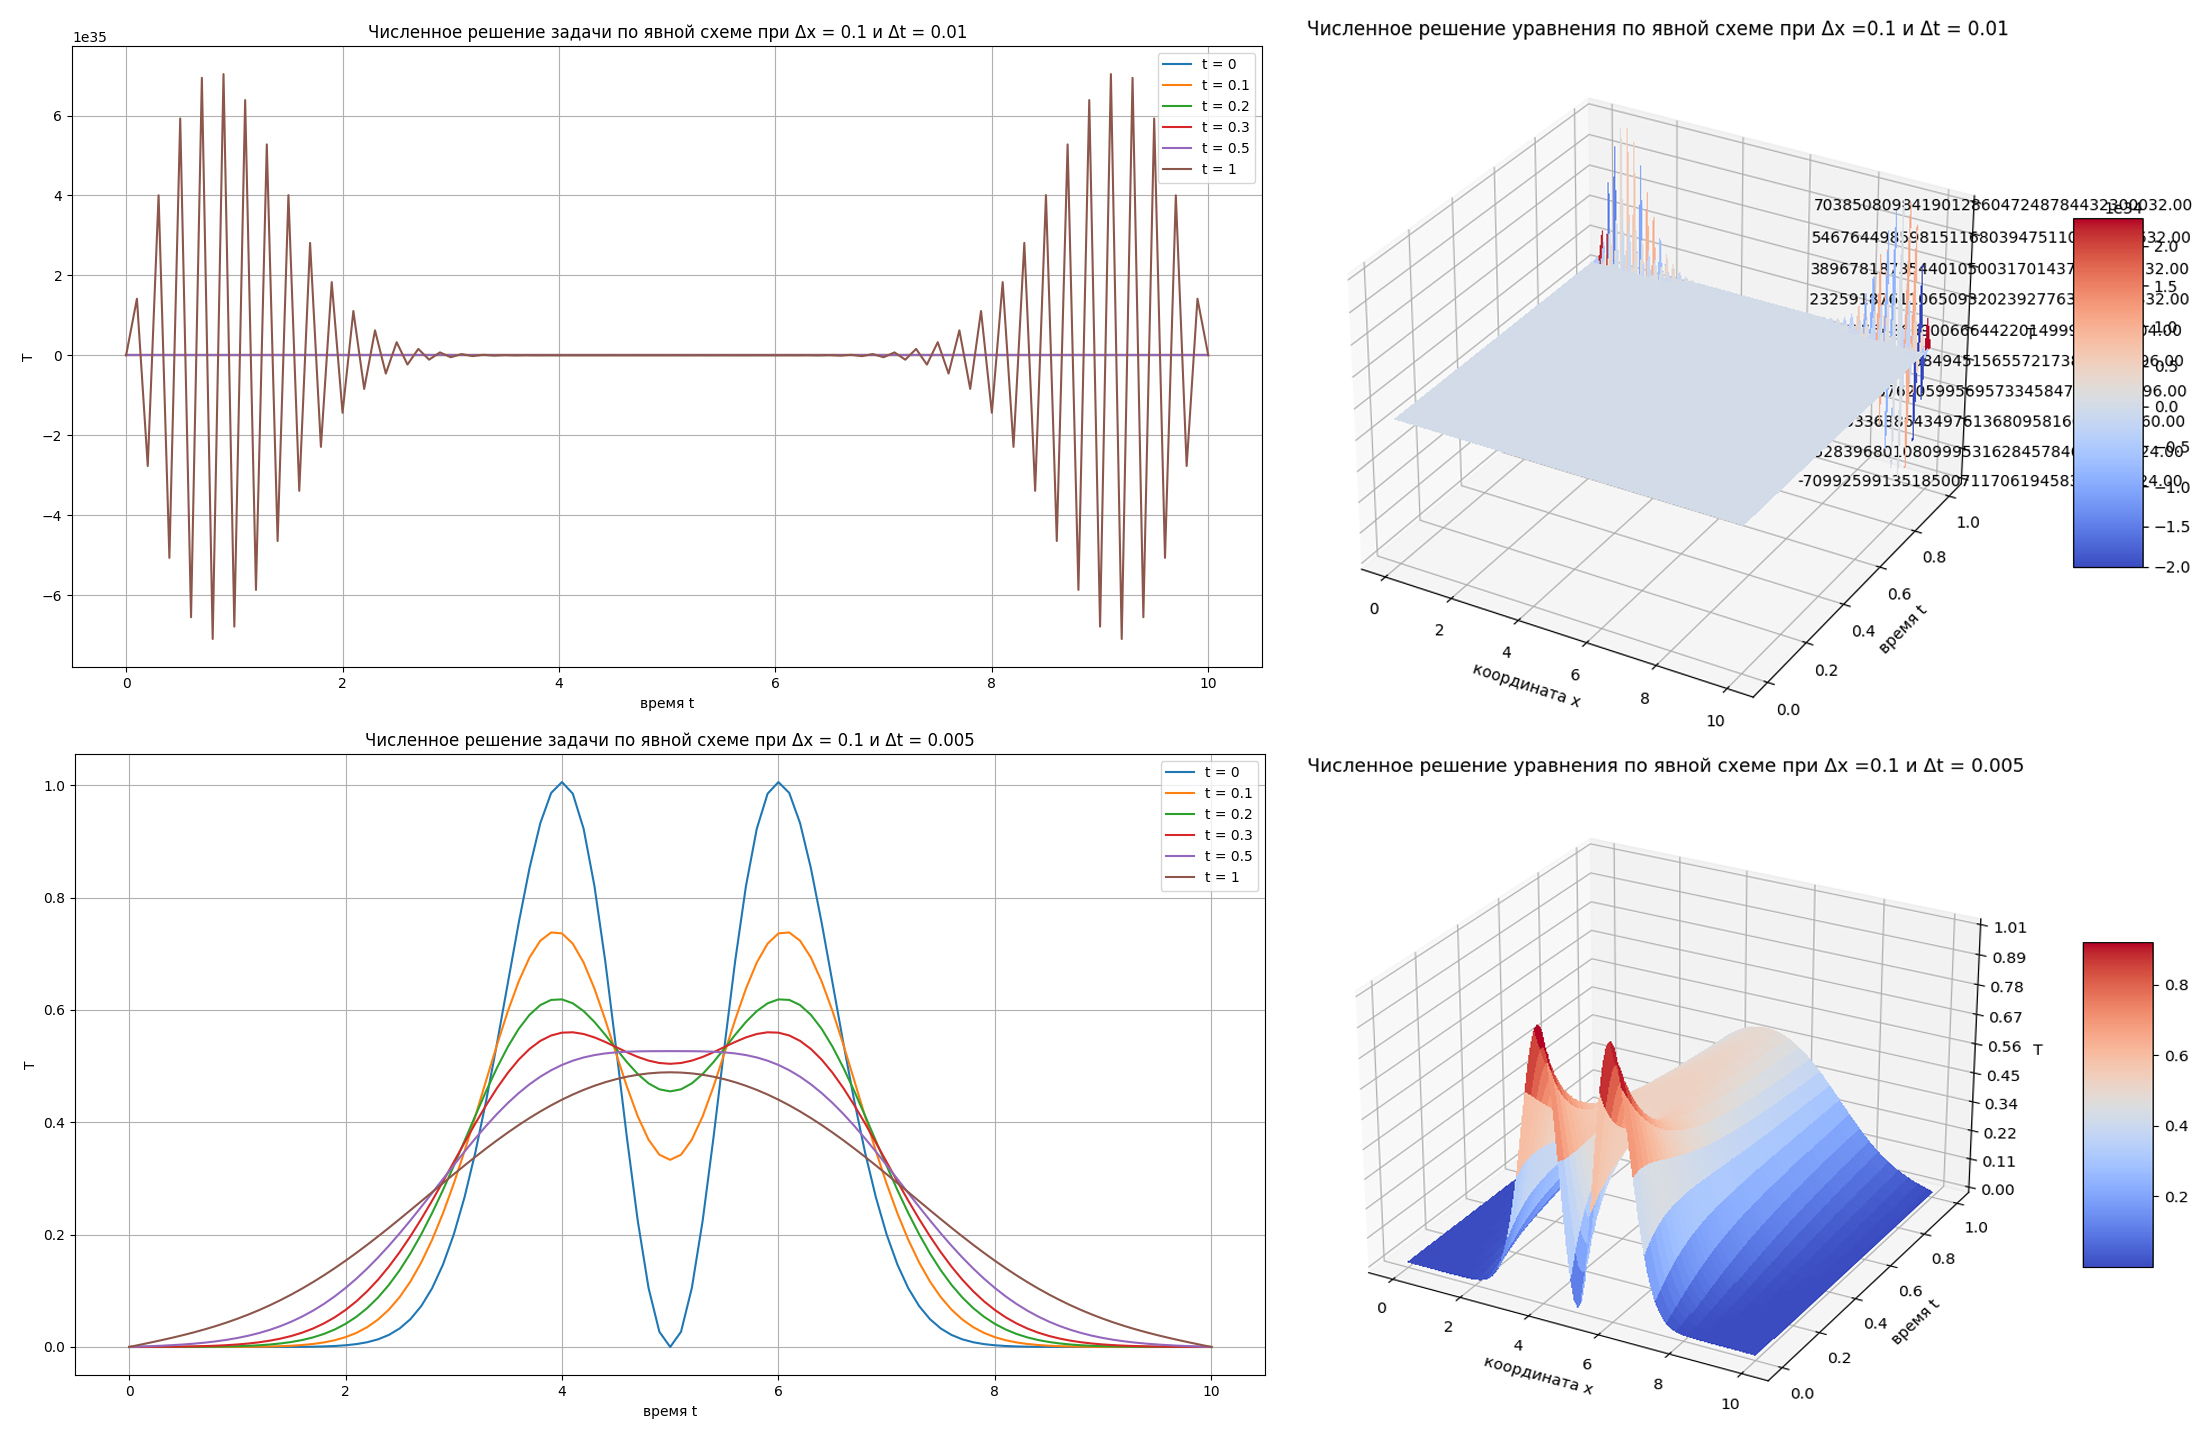
\includegraphics[scale=0.3]{j 1.jpg}
\caption{\label{pic2}  Численное решение по явной схеме при двух разных шагах сетки.}
\end{figure}

\begin{figure}[h!]
\centering
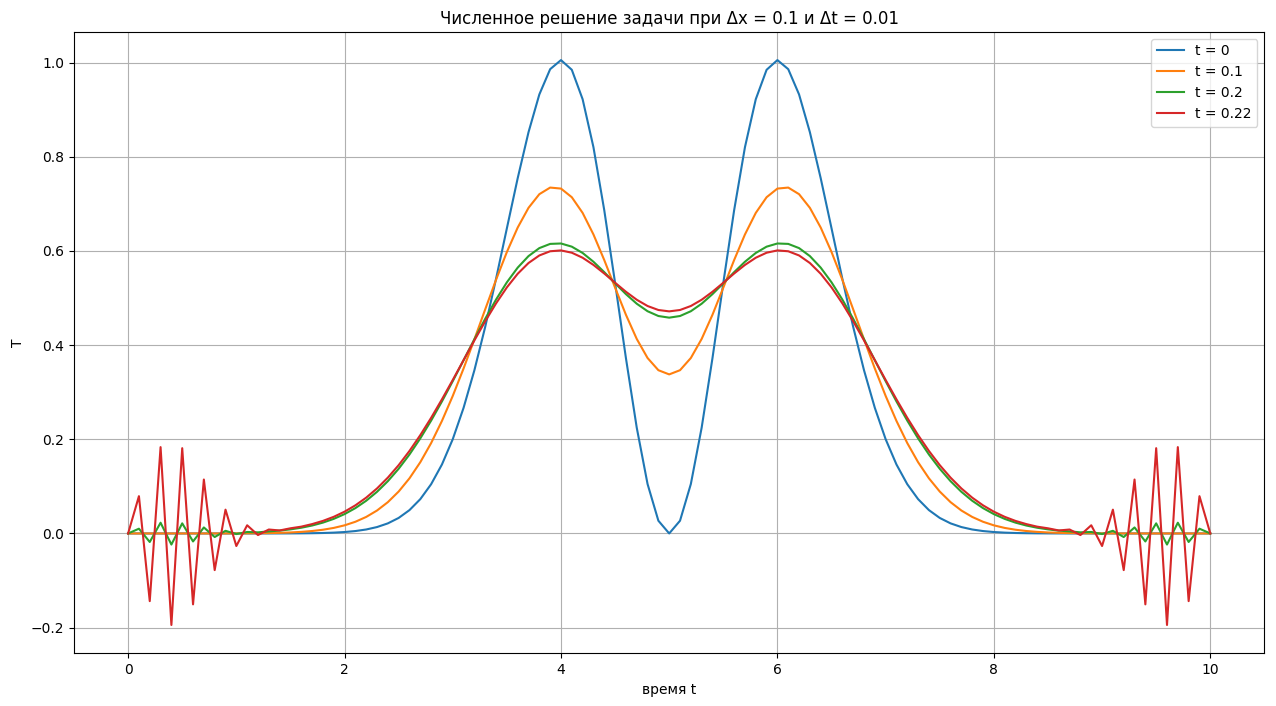
\includegraphics[scale=0.54]{neust.png}
\caption{\label{pic4}  Динамика развития неустойчивости.}
\end{figure}


\begin{figure}[h!]
\centering
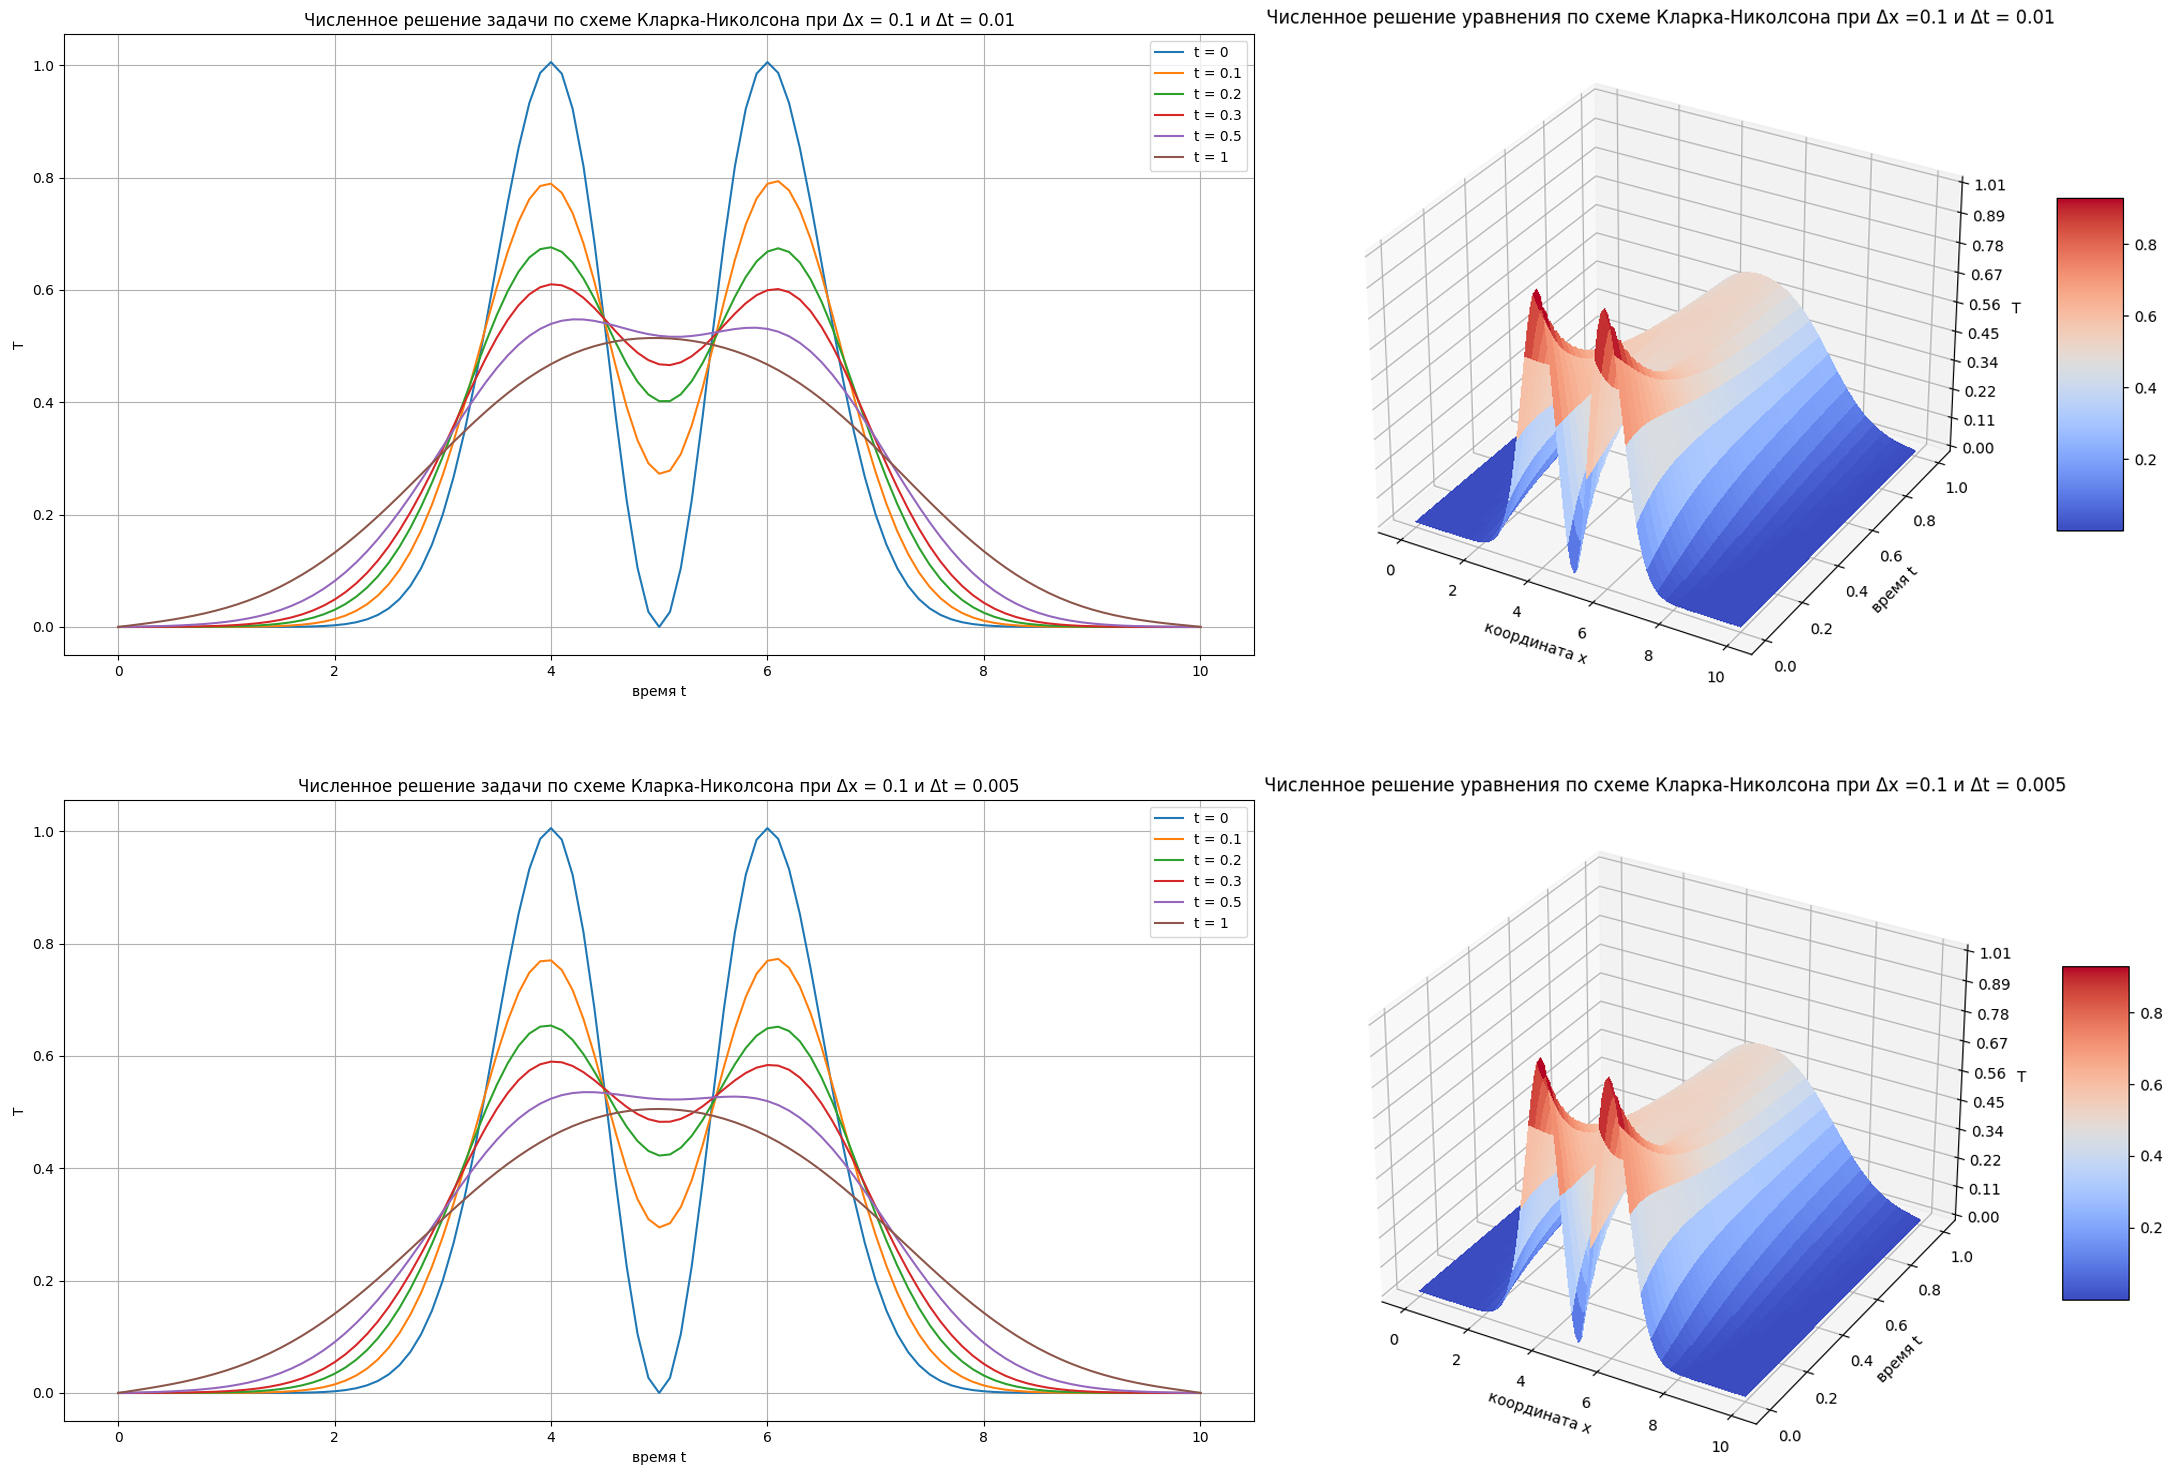
\includegraphics[scale=0.3]{n 1.jpg}
\caption{\label{pic3}  Численное решение по схеме Кранка-Николсона при двух разных шагах сетки.}
\end{figure}

Диффузия для обеих схем была также рассчитана для двух схем в теоретической части работы. Результаты представлены на рисунке \ref{pic5}. Синим изображены диффузии
непрерывного уравнения теплопроводности. Оранжевым построены сеточные
диффузии явной схемы и схемы Кларка-Николсона. 

Сеточная диффузия у схемы Кларка-Николсона имеет разрыв при частоте Найквиста, что сходится с теоретическим выражением. Действительно, при данных условиях на шаги при этом значении частоты знаменатель принимает нулевое значение, что и приводит к
разрыву. Для всех остальных случаев расположение разрывов также соответствуют уравнениям, выведенным в теории. 

\begin{figure}[h!]
\centering
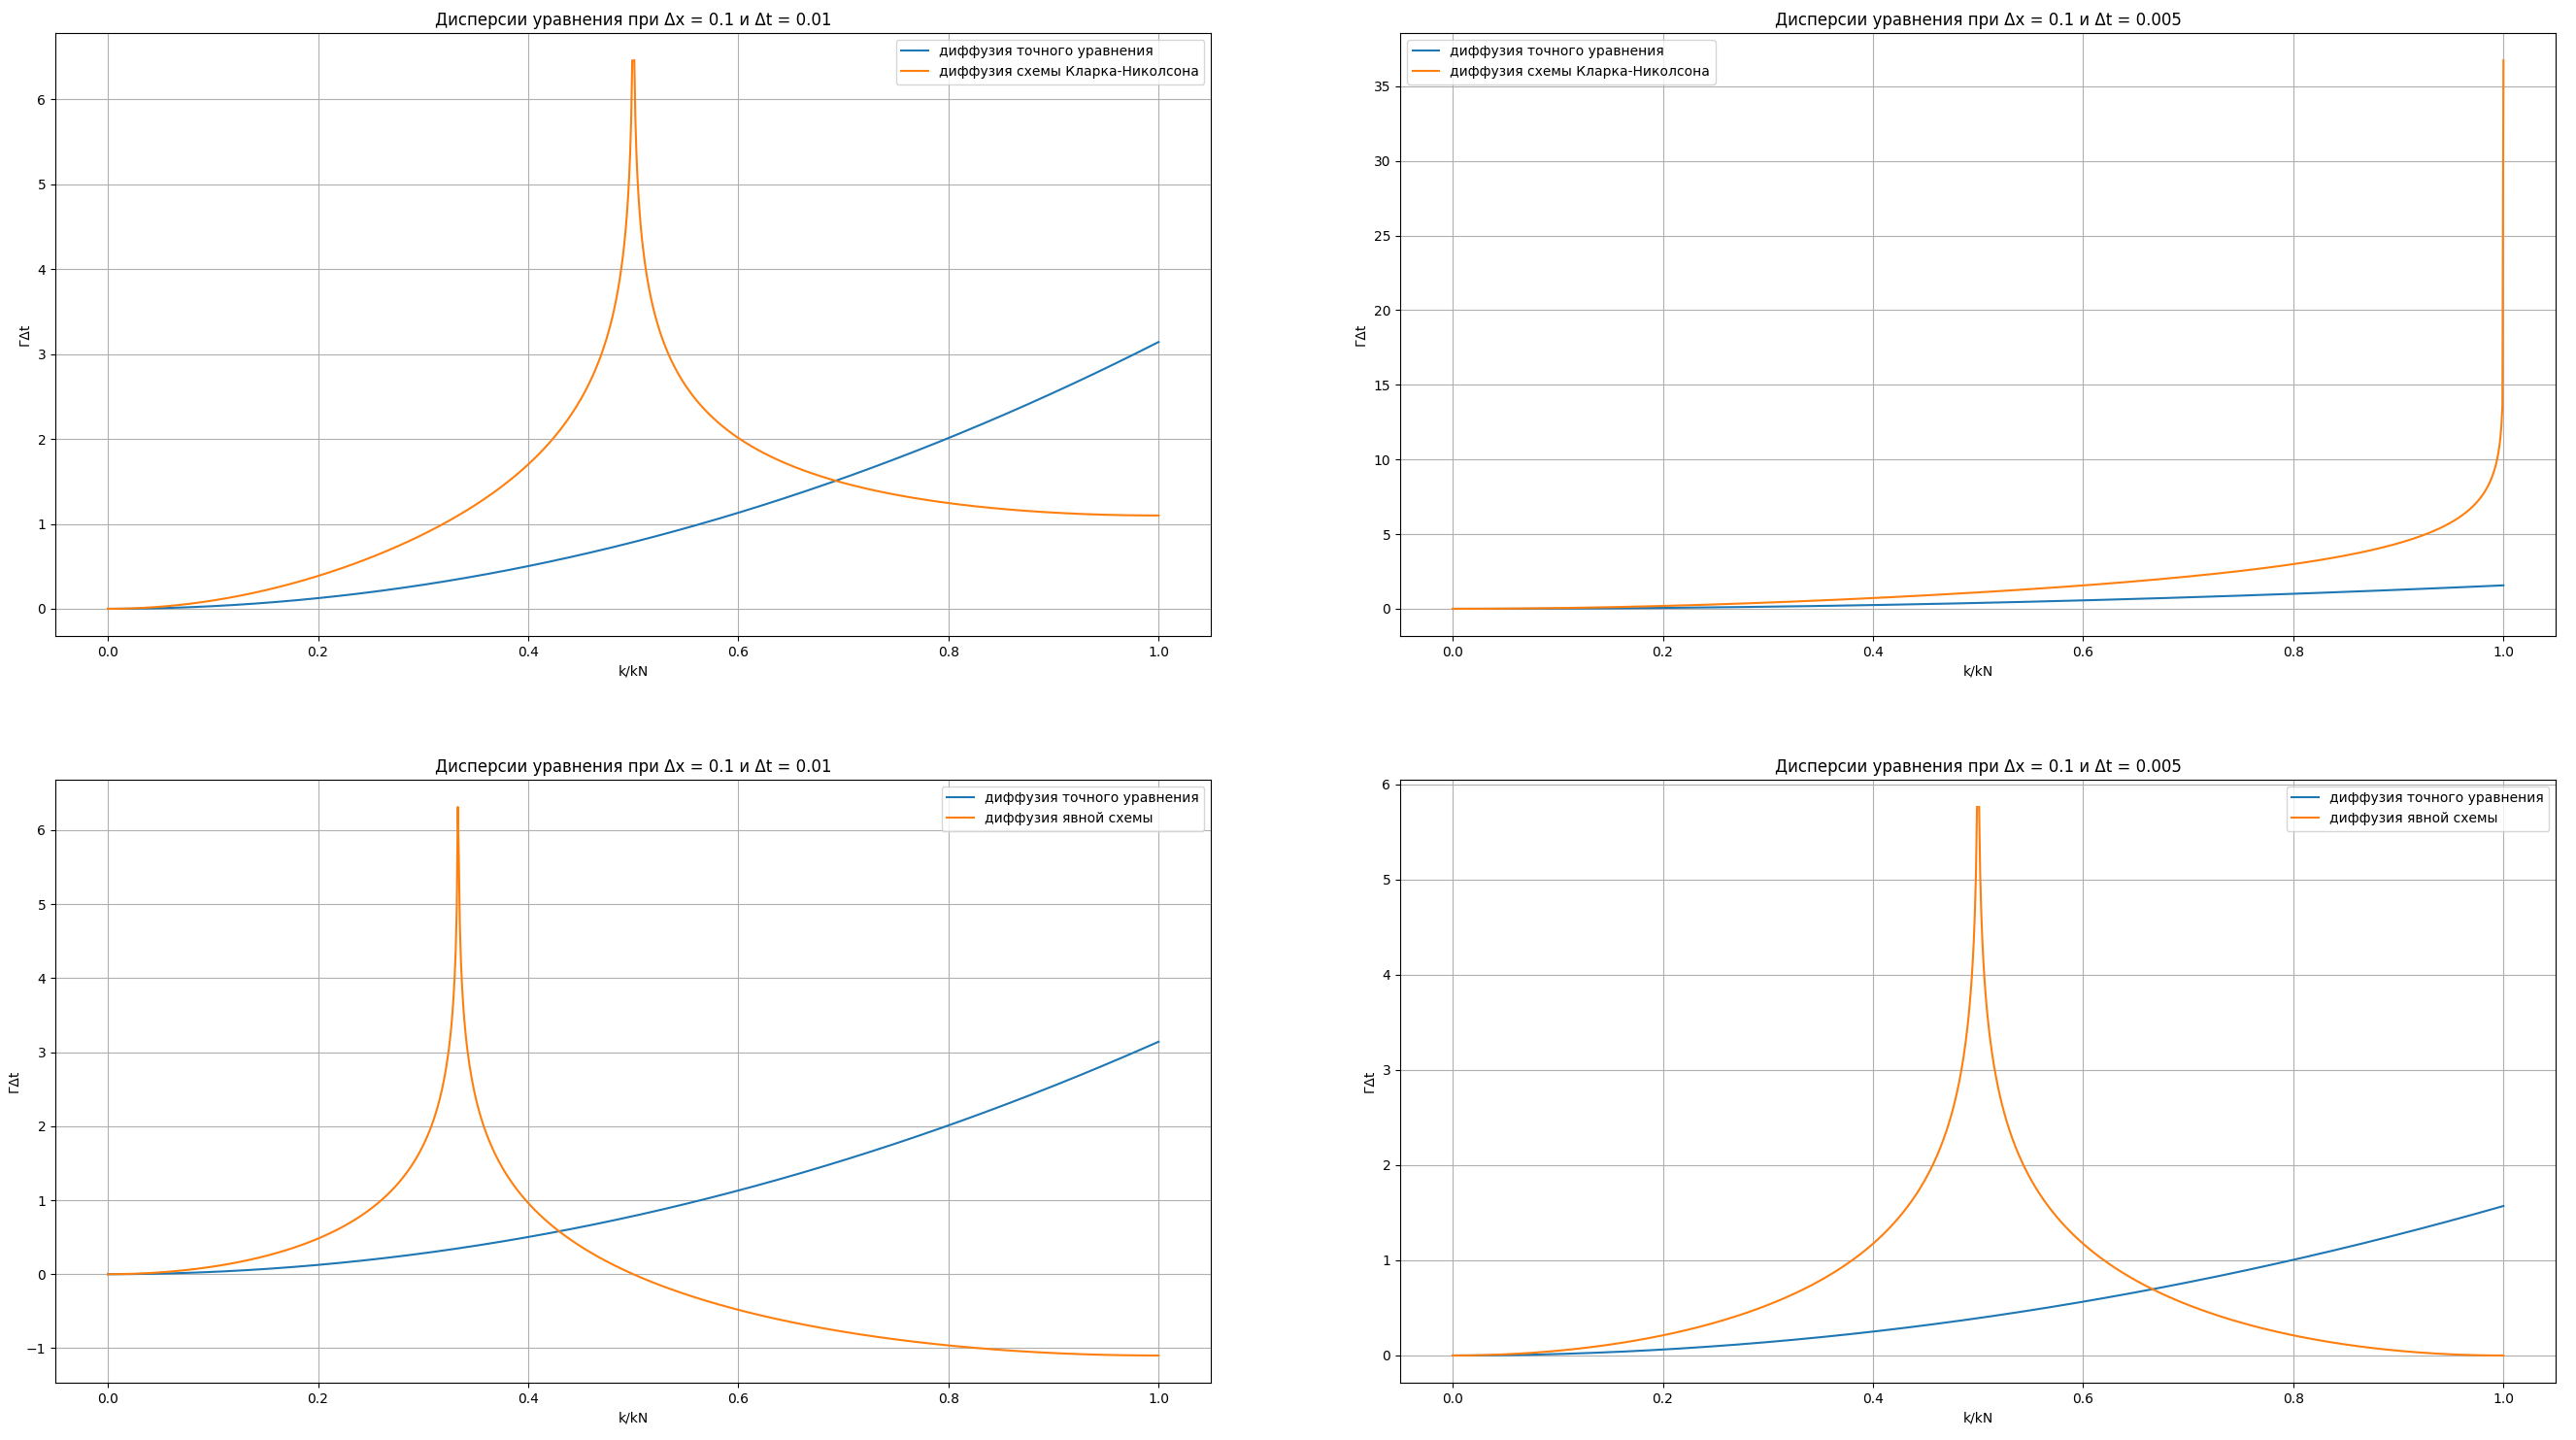
\includegraphics[scale=0.26]{D.jpg}
\caption{\label{pic5}  Диффузии разностных уравнений при разных шагах для разных схем в сравнении с диффузией точного уравнения.}
\end{figure}

\end{document}